\section* {3.1  Построение интерполяционных многочленов Лагранжа и Ньютона}

\subsection{Постановка задачи}
Используя таблицу значений $Y_i$ функции $y=f(x)$, вычисленных в точках $X_i, i=0,..3$ построить интерполяционные многочлены Лагранжа и Ньютона, проходящие через точки $\{X_i,Y_i \}$ . Вычислить значение погрешности интерполяции в точке $X^*$. 
 

{\bfseries Вариант:} 22

$y=arcctg(x)+x, a)X_i= -3,-1,1,3; б)X_i= -3,0,1,3;$
% \pagebreak

\subsection{Результаты работы}
\begin{figure}[h!]
\centering
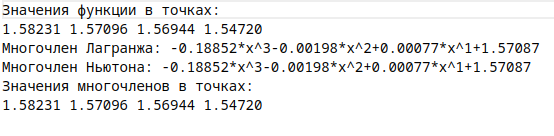
\includegraphics[width=.9\textwidth]{lab3.1}
\caption{Вывод программы в консоли}
\end{figure}

% \vfill

% \begin{figure}[h!]
% \centering
% \includegraphics[width=.9\textwidth]{lab5_taylor}
% \caption{Решение с аппроксимацией граничных условий со вторым порядком}
% \end{figure}
\pagebreak

\subsection{Исходный код}
% \lstinputlisting[language=C++]{matrix.cpp}
% \begin{lstlisting}
\lstinputlisting{include/lab3_1.cpp}
\lstinputlisting{include/interpolation.h}
\lstinputlisting{include/polynom.h}
% \end{lstlisting}
% \lstinputlisting{matrix.cpp}
% {../../include/matrix.cpp}
% \pagebreak
% \lstinputlisting[title=\texttt{parabolic\_pde.hpp}]{../../include/partial_differential/parabolic_pde.hpp}
% \pagebreak
% 